

Key-frame motion profiles for humanoids borrows from the animation industries' long used techniques.  
When making an animation the master artist/cartoonist will create the character in the most important (or key) poses.  
The apprentice will draw all of the frames between the key poses.  
We borrowed this technique when we: posed the robot in the desired pose, record the values in joint space, and make a smooth motion between poses.  
In place of the apprentice, forth order interpolation methods were used to make smooth trajectories between poses.  
Forth order interpolation was used in order to limit the jerk on each of the joints.  
The resulting trajectory is a smooth well defined motion as seen in Fig.~\ref{fig:keyframe-throw}.

\begin{figure}[t]
  \centering
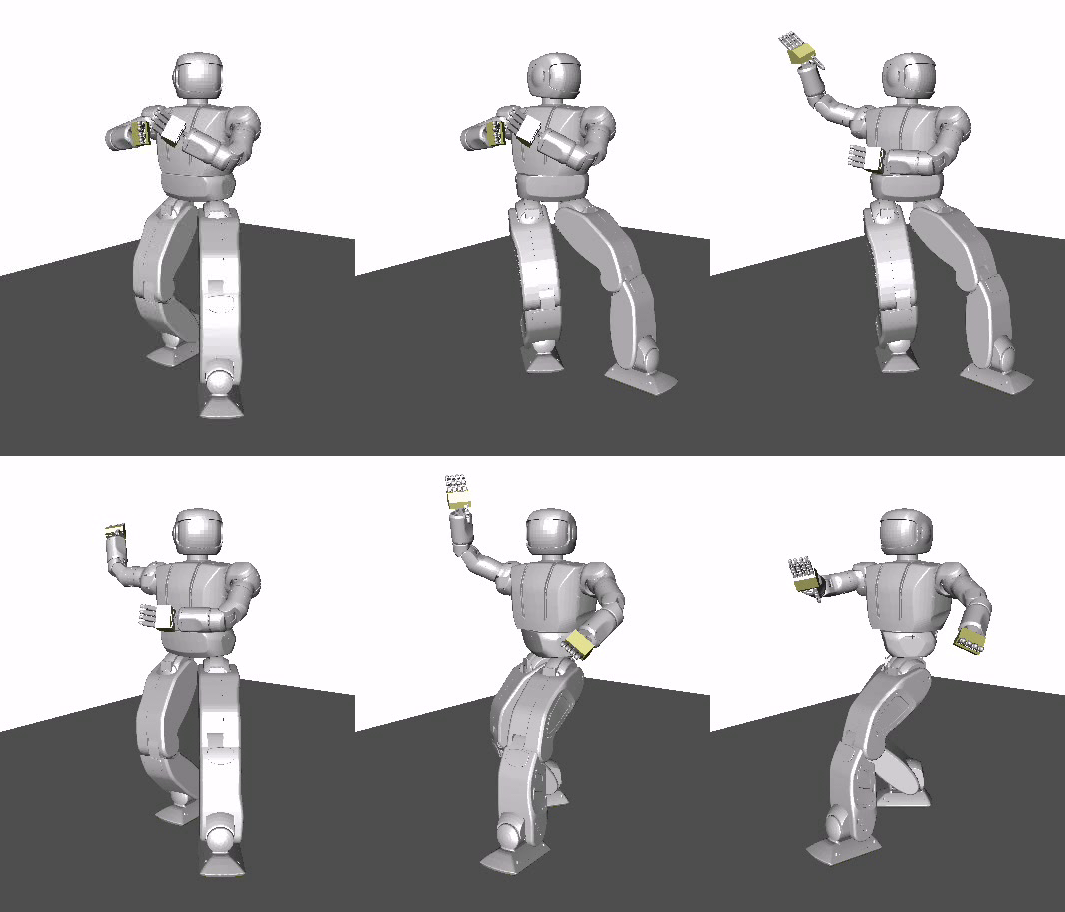
\includegraphics[width=0.8\columnwidth]{./pix/keyframe/keyframe.png}
  \caption{OpenHUBO using key-frame based method for throwing trajectory creation.  Frames are read from top left to bottom right.  Video of the above trajectory can be found at http://danlofaro.com/Humanoids2012/\#keyframe}
  \label{fig:keyframe-throw}
\end{figure}

To ensure stability throughout the motion the balance controller as described in Section~\ref{sec:sec:balance} was applied and the static ZMP criteria was checked for the entire trajectory.
The resulting end effector velocity was 4.8 $\frac{m}{s}$ at the release point.  
Fig.~\ref{fig:keyframe-graph} shows the plot of the magnitude of the end effector's velocity.  
It should be noted that at the instance of release the velocity vector is at an elevation of $40^o$ from the ground.

\begin{figure}[t]
  \centering
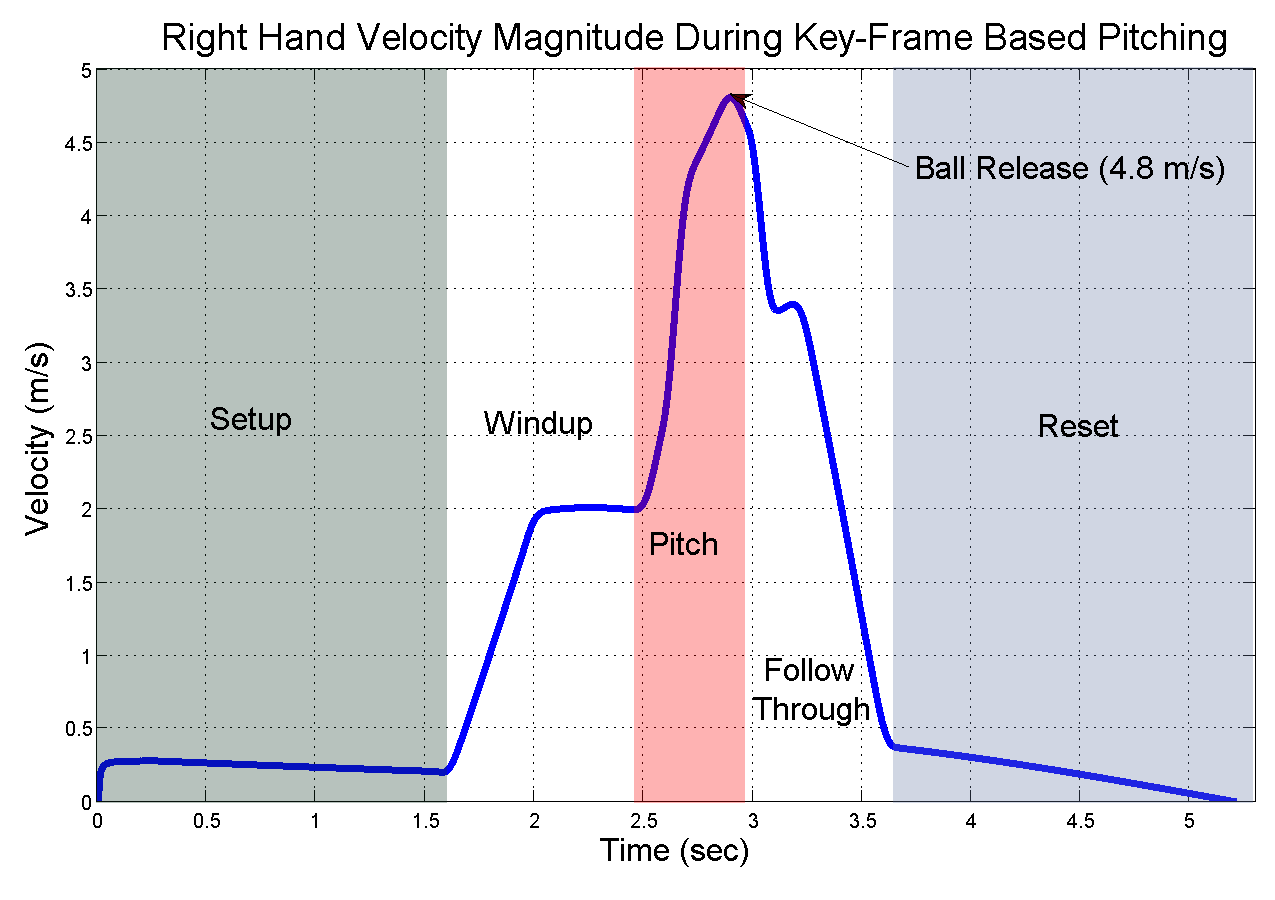
\includegraphics[width=1.0\columnwidth]{./fig/keyFrameThrow4.pdf}
  \caption{Velocity vs. Time graph showing the magnitude of the end-effector's velocity for the key-frame based throwing motion.  The six different stages of pitching are also shown.  Setup: move from the current position to th throw stance.  Windup: end effector starts to accelerate from the throw stance and move into position for the start of the pitch state. Pitch: end effector accelerates to release velocity.  Ball Release: the ball leaves the hand at maximum velocity (4.8 $\frac{m}{s}$) at an elevation of $40^o$ from the ground.  Follow Through: reducing velocity of end effector and all joints.  Reset: moves to a ready state for anther throw if needed.}
  \label{fig:keyframe-graph}
\end{figure}
